\documentclass[a4paper,twoside]{article}

\usepackage{epsfig}
\usepackage{subfigure}
\usepackage{calc}
\usepackage{amssymb}
\usepackage{amstext}
\usepackage{amsmath}
\usepackage{amsthm}
\usepackage{multicol}
\usepackage{pslatex}
\usepackage{apalike}
\usepackage{SCITEPRESS}
\usepackage[small]{caption}
\usepackage{booktabs}



\subfigtopskip=0pt
\subfigcapskip=0pt
\subfigbottomskip=6pt

\renewcommand{\arraystretch}{1.2}

\usepackage[english]{babel} 

% please place your own definitions here and don't use \def but
% \newcommand{}{}

\usepackage{latexsym}
\usepackage{amsmath,bm,amssymb}

\usepackage{tabularx}
\newcolumntype{C}{>{\centering\arraybackslash}X}
\usepackage{url}
\usepackage{subfigure}
% Use graphicx for including graphics
%\usepackage[dvips]{graphicx,psfrag}
\usepackage{graphicx}
\DeclareGraphicsExtensions{.eps}
\usepackage{paralist}

\renewcommand{\vec}[1]{\mathbf{#1}}
\newcommand{\vphi}{{\boldsymbol{\phi}}}
\newcommand{\Exp}{{\mathbb E}}
\newcommand{\inner}[2]{\big<{#1}\cdot{#2}\big>}
\newcommand{\norm}[1]{\lVert#1\rVert}

\usepackage[capitalise]{cleveref} % must come last

\newcommand{\phiproc}{$\phi_1$}
\newcommand{\phistartTime}{$\phi_2$}
\newcommand{\phiendTime}{$\phi_3$}
\newcommand{\phimacFree}{$\phi_4$}
\newcommand{\phimakespan}{$\phi_5$}
\newcommand{\phiwrmJob}{$\phi_6$}
\newcommand{\phiwrmMWR}{$\phi_7$}
\newcommand{\phislots}{$\phi_{8}$}
\newcommand{\phislotsTotal}{$\phi_{9}$}
\newcommand{\phislotsTotalperOp}{$\phi_{10}$}
\newcommand{\phiwait}{$\phi_{11}$}
\newcommand{\phislotCreated}{$\phi_{12}$}
\newcommand{\phitotProc}{$\phi_{13}$}
% schedule related

\begin{document}


\title{Evolutionary learning of weighted linear composite dispatching rules for scheduling}

\author{\authorname{Helga Ingimundardottir and Thomas Philip Runarsson }
\affiliation{Department of Industrial Engineering, Mechanical Engineering and Computer Science, \\University of Iceland, Hjardarhagi 2-6, IS-107 Reykjavik, Iceland.}
\email{\{hei2, tpr\}@hi.is}
}

\keywords{JOB SHOP SCHEDULING, COMPOSITE DISPATCHING RULES, EVOLUTIONARY SEARCH}

\abstract{A prevalent approach to solving job shop scheduling problems is to combine several relatively simple dispatching rules such that they may benefit each other for a given problem space. Generally, this is done in an ad-hoc fashion, requiring expert knowledge from heuristics designers, or extensive exploration of suitable combinations of heuristics. The approach here is to automate that selection by translating dispatching rules into measurable features and optimising what their contribution should be via evolutionary search. The framework is straight forward and easy to implement and shows promising results. Various data distributions are investigated for both job shop and flow shop problems, as is scalability for higher dimensions. 
Moreover, the study shows that the choice of objective function  for evolutionary search is worth investigating. Since the optimisation is based on minimising the expected mean of the fitness function over a large set of problem instances which can vary within the set, then normalising the objective function can stabilise the optimisation process away from local minima. 
}

\onecolumn \maketitle \normalsize \vfill

\section{\uppercase{Job shop scheduling}}
The job-shop scheduling problem (JSP) deals with the allocation of tasks of competing resources where the goal is to optimise a single or multiple objectives -- in particular minimising a schedule's maximum completion time, i.e., the makespan, denoted $C_{\max}$. Due to difficulty in solving this problem, heuristics are generally applied. Perhaps the simplest approach to generating good feasible solutions for JSP is by applying dispatching rules (DR),  e.g., choosing a task corresponding to longest or shortest processing time, most or least successors, or ranked positional weight, i.e., sum of processing times of its predecessors. Ties are broken in an arbitrary fashion or by another heuristic rule. Combining dispatching rules for JSP is promising, however, there is a large number of rules to choose from, thus its combinations rely on expert knowledge or extensive trial-and-error process to choose a suitable DR \cite{Tay08}. Hence given the diversity within the JSP paradigm, there is no ``one-rule-fits-all'' for all problem instances (or shop constraints), however single priority dispatching rules (SDR) based on job processing attributes have proven to be effective~\cite{Haupt89}. 
The classical dispatching rules are continually used in research; a summary of over $100$ classical DRs for JSP can be found in \cite{Panwalkar77}. 
However, careful combinations of such simple rules, i.e., composite dispatching rules (CDRs) can perform significantly better \cite{Jayamohan04}. 
As a consequence, a linear composite of dispatching rules for JSP was presented in \cite{InRu11a}. There the goal was to learn a set of weights, $\vec{w}$ via ordinal regression such that 
\begin{equation}\label{eq:jssp:linweights}
h(\vec{x}_j)=\inner{\vec{w}}{\vphi(\vec{x}_j)},
\end{equation}
yields the preference estimate for dispatching job $j$ that corresponds to post-decision state $\vec{x}_j$, where $\vphi(\vec{x}_j)$ denotes the feature mapping (cf.~\cref{sec:feat}). 
In short, \cref{eq:jssp:linweights} is a simple linear combination of features found using a classifier which is trained by giving more weight to instances that are preferred w.r.t. optimality in a supervised learning fashion. As a result, the job dispatched is the following, 
\begin{equation}\label{eq:jstar}
j^* = \arg\max_j\left\{h(\vec{x}_j)\right\}. 
\end{equation}

A more popular approach in recent JSP literature is applying genetic algorithms (GAs)~\cite{Pinedo08}. However, in that case an extensive number of schedules need to be evaluated, and even for low dimensional JSP, it can quickly become computationally infeasible.
GAs can be used directly on schedules~\cite{Cheng96,Cheng99,Tsai07,Qing-dao-er-ji12,Ak12}, however, then there are many concerns that need to be dealt with. To begin with there are nine encoding schemes for representing the schedules~\cite{Cheng96}, in addition, special care must be taken when applying cross-over and mutation operators in order for schedules to still remain feasible. Moreover, in case of JSP, GAs are not adapt for fine-tuning around optima. Luckily a subsequent local search can mediate the optimisation~\cite{Cheng99}.

The most predominant approach in hyper-heuristics, a framework of creating \emph{new} heuristics from a set of  predefined heuristics, is genetic programming~\cite{Burke10}. 
Dispatching rules based genetic algorithms (DRGA)~\cite{Vazquez-Rodriguez09,Dhingra10,Nguyen13} are a special case of genetic programming~\cite{Koza05}, where GAs are applied indirectly to JSP via dispatching rules, i.e., where a solution is no longer a \emph{proper} schedule but a \emph{representation} of a schedule via applying certain DRs consecutively. 

There are two main viewpoints on how to approach scheduling problems,
\begin{inparaenum}[\itshape a\upshape)] 
\item local level by building schedules for one problem instance at a time;
and \item global level by building schedules for all problem instances at once.
\end{inparaenum}
For local level construction a simple construction heuristic is applied. The schedule's features are collected at each dispatch iteration from which a learning model will inspect the feature set to discriminate which operations are preferred to others via ordinal regression. The focus is essentially on creating a meaningful preference set composed of features and their ranks as the learning algorithm is only run once to find suitable operators for the value function. This is the approach taken in~\cite{InRu11a}. Expanding on that  work, this study will explore a global level construction viewpoint where there is no feature set collected beforehand since the learning model is optimised directly via evolutionary search. This involves numerous costly value function evaluations. In fact it involves an indirect method of evaluation whether one learning model is preferable to another, w.r.t. which one yields a better expected mean. 

\section{\uppercase{Outline}}
In order to formulate the relationship between problem structure and heuristic efficiency, one can utilise Rice's framework for algorithm selection ~\cite{Rice76}. The framework consists of four fundamental components, namely,
\vfill
\begin{description}
  \item[Problem space or instance space] $\mathcal{P}$, \hfill\\
  set of problem instances; 
  \item[Feature space] $\mathcal{F}$, \hfill\\
  measurable properties of the instances in $\mathcal{P}$;
  \item[Algorithm space] $\mathcal{A}$, \hfill\\
  set of all algorithms under inspection;
  \item[Performance space] $\mathcal{Y}$, \hfill\\
  the outcome for $\mathcal{P}$ using an algorithm from $\mathcal{A}$.
\end{description}
\vfill
For a given problem instance $\vec{x}\in\mathcal{P}$ with $k$ features $\vphi(\vec{x})=\{\phi_1(\vec{x}),...,\phi_k( \vec{x})\}\in\mathcal{F}$ and using algorithm $a\in\mathcal{A}$ the performance is $y=Y(a,\vphi(\vec{x}))\in\mathcal{Y}$, where $Y:\;\mathcal{A}\times\mathcal{F} \mapsto \mathcal{Y}$ is the mapping for algorithm and feature space onto the performance space. 
\cite{SmithMilesLion3,SmithMilesLion5,InRu12} formulate JSP in the following manner: 
\begin{inparaenum}[\itshape a\upshape)] 
\item problem space $\mathcal{P}$ is defined as the union of $N$ problem instances consisting of processing time and ordering matrices given in~\cref{sec:data}; 
\item feature space $\mathcal{F}$, which is outlined in~\cref{sec:feat}. Note, these are not the only possible set of features, however, they are built on the work by~\cite{InRu11a,SmithMilesLion3} and deemed successful in capturing the essence of a JSP data structure;
\item algorithm space $\mathcal{A}$ is simply the scheduling policies under consideration and discussed in~\cref{sec:expr};
\item performance space is based on the resulting $C_{\max}$. Different fitness measures are investigated in~\cref{sec:expr:measure};
and \item mapping $Y$ is the step-by-step scheduling process. 
\end{inparaenum}

In the context of Rice's framework, and returning to the aforementioned approaches to scheduling problems, then the objective is to maximise its expected heuristic performance, i.e.,
\begin{enumerate}[\itshape a\upshape)] 
\item Local level 
\begin{equation}
\max_{\mathcal{P}'\subset\mathcal{P}}~\mathbb{E}\left[Y\left(a,\vphi(\vec{x})\right)\right]
\end{equation}
where $\vec{x}\in\mathcal{P}'$ and algorithm $a$ is obtained via ordinal regression based on the feature space $\mathcal{F}$, i.e., $\mathcal{F}|_{\mathcal{P}'}\mapsto\mathcal{A}$, such as the approach taken in~\cite{InRu11a}, and  will be used as a benchmark for the following,  
%In addition, for global level,
\item  Global level
\begin{equation}
\max_{a\in\mathcal{A}}~\mathbb{E}\left[Y\left(a,\vphi(\vec{x})\right)\right]
\end{equation}
where training data $\vec{x}\in\mathcal{P}$ is guided by its algorithm $a$, i.e., $\mathcal{A}\mapsto\mathcal{P}$. This will be the focus of this study.
\end{enumerate}
Note that the mappings $\vphi:\mathcal{P}\mapsto\mathcal{F}$ and $Y:\mathcal{A}\mapsto\mathcal{Y}$ are the same for both paradigms.

The paper concludes in~\cref{sec:disc} with discussion and conclusions.

\section{\uppercase{Problem space}}\label{sec:data}
For this study synthetic JSP and its subclass, permutation flow shop problem (PFSP), the scheduling task considered here is where $n$ jobs are scheduled on a set of $m$ machines, i.e., problem size $n\times m$, subject to the constraint that each job must follow a predefined machine order and that a machine can handle at most one job at a time. The pair $(j,a)$ refers to the operation of dispatching job $j$ on machine $a$. As a result, a total of $\ell = n\cdot m$ sequential operations need to be made for a complete schedule.

The objective is to schedule the jobs so as to minimize the maximum completion times, $C_{\max}$, also known as the makespan.  For a mathematical formulation of JSP the reader is recommended \cite{InRu11a}. 

There are two fundamental types of problem classes: non-structured versus structured. 
Firstly there are the ``conventional'' structured problem classes, where problem instances are generated stochastically by fixing the number of jobs and machines, as well as processing times are i.i.d. and sampled from a discrete uniform distribution from the interval $I=[u_1,u_2]$, i.e., $p\sim \mathcal{U}(u_1,u_2)$.
Two different processing time distributions are explored, namely 
$\mathcal{P}_{j.rnd}$ where $I=[1,99]$ and $\mathcal{P}_{j.rndn}$ where $I=[45,55]$, referred to as random and random-narrow, respectively.
The machine order is a random permutation of all of the machines in the job-shop. 

Analogous to $\mathcal{P}_{j.rnd}$ and $\mathcal{P}_{j.rndn}$ the problem classes $\mathcal{P}_{f.rnd}$ and $\mathcal{P}_{f.rndn}$, respectively, correspond to the structured PFSP problem classes, however with a homogeneous machine order permutation.  
Secondly, there are structured problem classes of PFSP which are modelled after real-world flow-shop manufacturing namely job-correlated $\mathcal{P}_{f.jc}$ where job processing times are dependent on job index and independent of machine index.
Problem instances for PFSP are generated using~\cite{Whitley} problem generator\footnote{Both code, written in \texttt{C++}, and problem instances used in their experiments can be found at: \url{http://www.cs.colostate.edu/sched/generator/}}. 

For each JSP and PFSP class $N_{\text{train}}$  and $N_{\text{test}}$ instances were generated for training and testing, respectively. Values for $N$ are given in~\cref{tbl:data:sim}. Note, difficult problem instances are not filtered out beforehand, such as the approach in~\cite{Whitley}. 


\begin{table}\centering
\caption{Problem space distributions used in~\cref{sec:expr}. Note, problem instances are synthetic and each problem space is i.i.d. and `--' denotes not available.}\label{tbl:data:sim}
{\renewcommand{\arraystretch}{1.5}
\begin{tabularx}{\columnwidth}{l|c|C|C|l}\toprule
name&size & $N_{\text{train}}$&$N_{\text{test}}$  & note 
\\  \midrule
\multicolumn{5}{c}{Permutation flow shop problem (PFSP)} \\ \midrule
%\multirow{6}{*}{\begin{sideways}PFSP\end{sideways}}
$\mathcal{P}_{f.rnd}^{6\times5}$ &$6\times5$& 500&--& random \\ 
$\mathcal{P}_{f.rndn}^{6\times5}$&$6\times5$& 500&--& random-narrow \\ 
$\mathcal{P}_{f.jc}^{6\times5}$  &$6\times5$& 500&--& job-correlated \\ 
$\mathcal{P}_{f.rnd}^{10\times10}$ &$10\times10$&--&500&random \\ 
$\mathcal{P}_{f.rndn}^{10\times10}$&$10\times10$&--&500& random-narrow \\ 
$\mathcal{P}_{f.jc}^{10\times10}$  &$10\times10$&--&500& job-correlated \\ 
\midrule
\multicolumn{5}{c}{Job shop problem (JSP)} \\ \midrule
%\multirow{4}{*}{\begin{sideways}JSP\end{sideways}}
$\mathcal{P}_{j.rnd}^{6\times5}$ & $6\times5$ & 500 & -- & random \\
$\mathcal{P}_{j.rndn}^{6\times5}$ & $6\times5$ & 500 & -- & random-narrow \\
$\mathcal{P}_{j.rnd}^{10\times10}$ &$10\times10$& -- & 500 & random \\
$\mathcal{P}_{j.rndn}^{10\times10}$ &$10\times10$& -- & 500 & random-narrow \\ 
\bottomrule
\end{tabularx}
}
\end{table}




\section{\uppercase{Feature space}}\label{sec:feat}
When building a complete JSP schedule, a job is placed at the earliest available time slot for its next machine while still fulfilling constraints that each machine can handle at most one job at a time, and jobs need to have finished their previous machines according to its machine order. 
Unfinished jobs are dispatched one at a time according to some heuristic. After each dispatch the schedule's current features are updated.
Features are used to grasp the essence of the current state of the schedule. As seen in~\cref{tbl:jssp:feat}, temporal scheduling features applied in this study are given for each possible post-decision state. An example of a schedule being built is given in~\cref{fig:jssp:example}, where there are a total of five possible jobs that could be chosen to be dispatched by some dispatching rule. These features would serve as the input for~\cref{eq:jssp:linweights}. 

It's noted that some of the features directly correspond to a SDR commonly used in practice. For example, if the weights $\vec{w}$ in~\cref{eq:jssp:linweights} were all zero, save for $w_6=1$, then~\eqref{eq:jstar} yields the job with the highest \phiwrmJob\ value, i.e., equivalent  to dispatching rule most work remaining (MWR).


\begin{table}  
  \caption{Feature space $\mathcal{F}$ for $\mathcal{P}$ given the resulting temporal schedule after dispatching an operation $(j,a)$.  }
  \label{tbl:jssp:feat}

\centering
  \begin{tabular}{ll} %p{0.45\textwidth}|p{0.4\textwidth}|}
\toprule
  $\vphi$ & Feature description \\
\midrule
  \phiproc & job $j$ processing time \\
  \phistartTime & job $j$ start-time \\
  \phiendTime & job $j$ end-time\\
  \phimacFree & when machine $a$ is next free \\
  \phimakespan & current makespan \\   
  \phiwrmJob & total work remaining for job $j$ \\
  \phiwrmMWR & most work remaining for all jobs\\
  \phislots & total idle time for machine $a$ \\
  \phislotsTotal & total idle time for all machines \\
  \phislotsTotalperOp & \phislotsTotal\ weighted w.r.t. number of assigned tasks\\
  \phiwait & time job $j$ had to wait \\
  \phislotCreated & idle time created \\      
  \phitotProc & total processing time for job $j$ \\
\bottomrule
  \end{tabular}

 %Feature description for job $J_j$ on machine $M_a$ given current temporal schedule, where the set of jobs already dispatched are $J\subset\mathcal{J}$ on corresponding set of machines $\mathcal{M}_j\subset\mathcal{M}$


\end{table}

\begin{figure*}[t!]\centering 
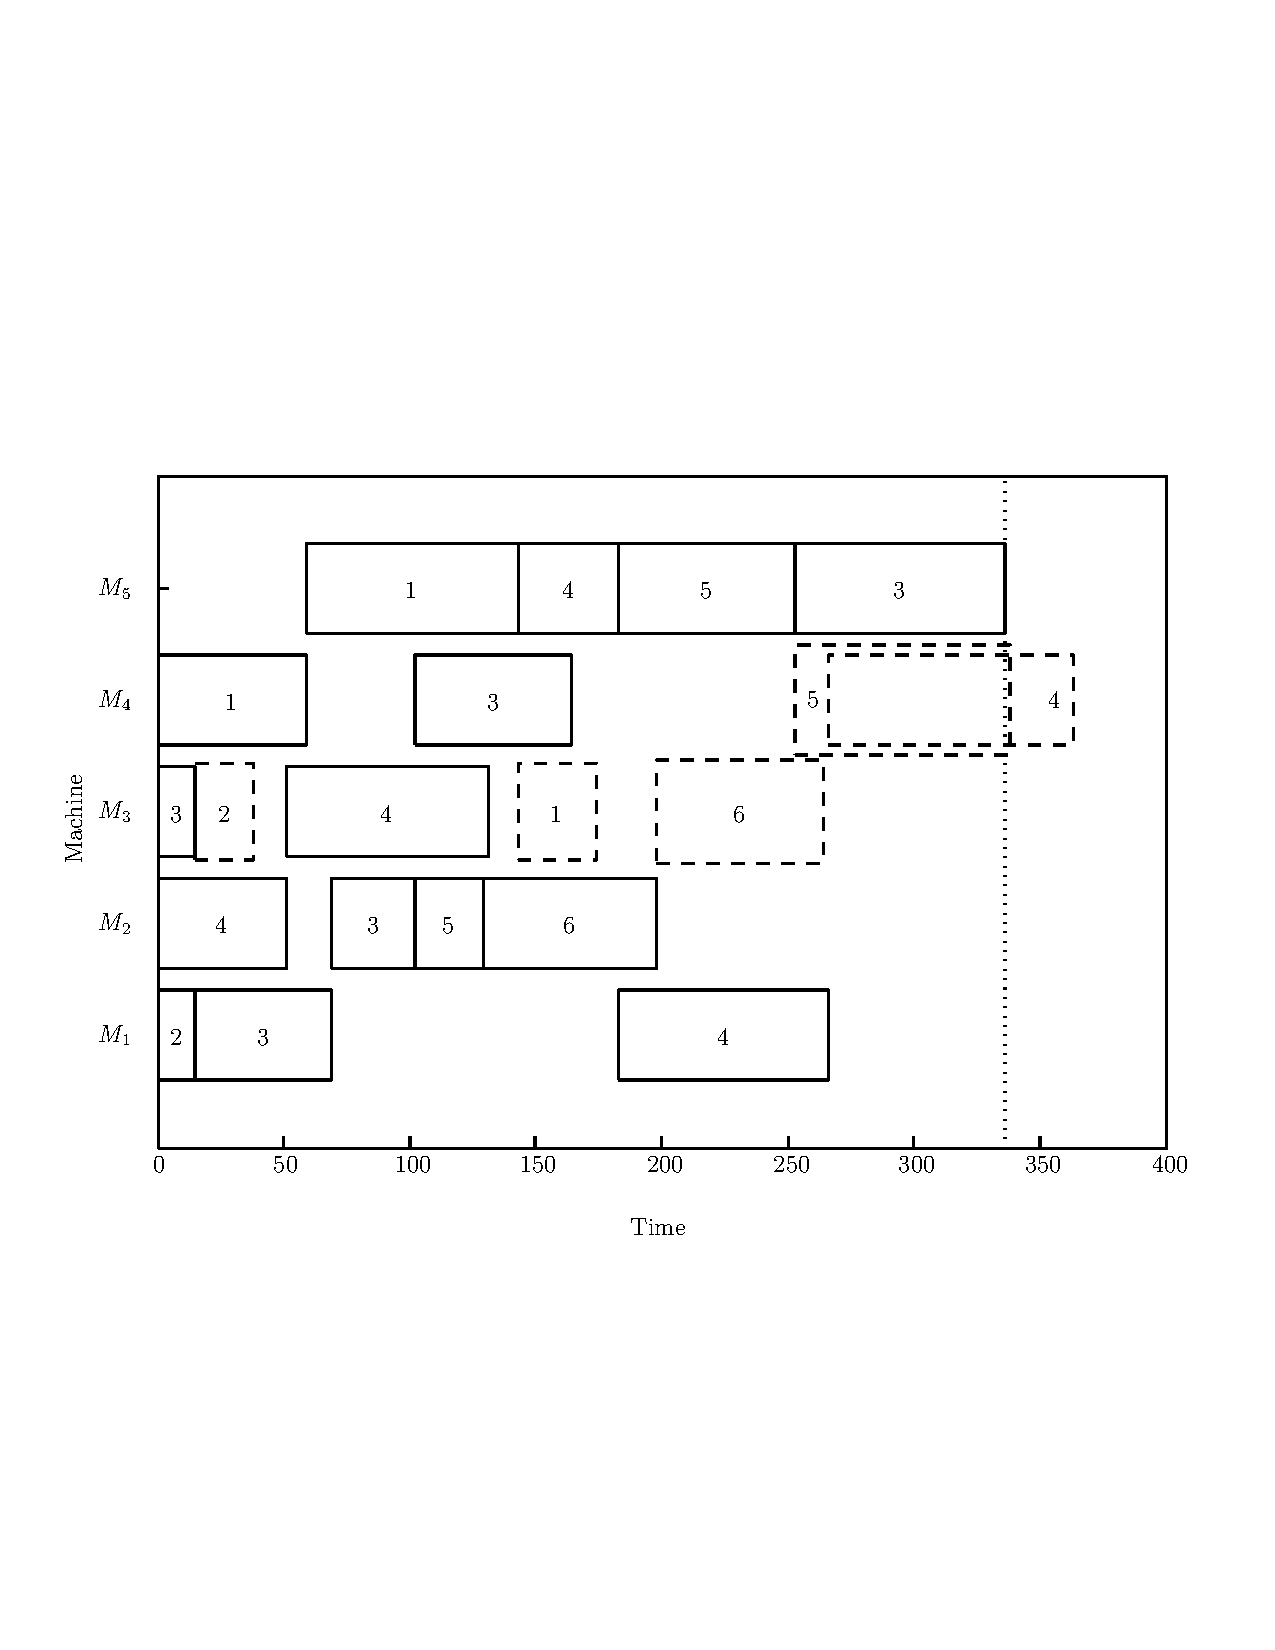
\epsfig{file=fig/jssp_example_nocolor, width=1.3\columnwidth}
\caption[Gantt chart of a partial JSP schedule]{Gantt chart of a partial JSP schedule after 15 operations: Solid boxes represent previously dispatched jobs, and dashed boxes represent  the jobs
that could be scheduled next. Current $C_{\max}$ denoted as dotted line.}
\label{fig:jssp:example}
\end{figure*}


\section{\uppercase{Experimental study}}\label{sec:expr}
The optimum makespan\footnote{Optimum values are obtained by using a commercial software package \cite{gurobi}.} is denoted 
$C_{\max}^{\text{opt}}$, and the makespan obtained from the heuristic model by $C_{\max}^{\text{model}}$. Since 
the optimal makespan varies between problem instances the performance measure is the following, 
\begin{equation}\label{eq:ratio}\rho :=\frac{C_{\max}^{\text{model}}-C_{\max}^{opt}}{C_{\max}^{\text{opt}}}\cdot 
100\%\end{equation}
which indicates the percentage relative deviation from optimality. Throughout a Kolmogorov-Smirnov test with $\alpha=0.05$ is applied to determine statistical significance between methodologies. 

Inspired by DRGA, the approach taken in this study is to optimise the weights $\vec{w}$ in~\cref{eq:jssp:linweights} directly via evolutionary search such as covariance matrix adaptation evolution strategy (CMA-ES) \cite{Hansen01}. This has been proven to be a very efficient numerical optimisation technique. 

Using standard set-up of parameters of the CMA-ES optimisation, the runtime was limited to 288 hours on a cluster for each training set given in~\cref{sec:data} and in every case the optimisation reached its maximum walltime.

\subsection{Performance measures}\label{sec:expr:measure}
Generally, evolutionary search only needs to minimise the expected fitness value. However, the  approach in~\cite{InRu11a} was to use the known optimum to correctly label which operations' features were optimal when compared to other possible operations. Therefore, it would be of interest to inspect if there is any performance edge gained by incorporating optimal labelling in evolutionary search. Therefore, two objective functions will be considered, namely, 
\begin{equation}
ES_{C_{\max}} := \min \Exp[C_{\max}] \label{eq:cma:makespan}
\end{equation}
\begin{equation}
ES_{\rho} := \min \Exp[\rho] \label{eq:cma:rho}
\end{equation} 
Main statistics of the experimental run are given in~\cref{cma:funeval} and depicted in~\cref{fig:cma:fit} for both approaches. In addition, evolving decision variables, here weights $\vec{w}$ for~\cref{eq:jssp:linweights}, are depicted in~\cref{fig:cma:wei}. 

In order to compare the two objective functions, the best weights reported were used for~\cref{eq:jssp:linweights} on the corresponding training data. Its box-plot of percentage relative deviation from optimality, defined by~\cref{eq:ratio}, is depicted in~\cref{fig:cma:trainboxpl} and \cref{tbl:results:train} present its main statistics; mean, median, standard deviation, minimum and maximum values.

In the case of $\mathcal{P}_{f.rndn}$,~\cref{eq:cma:makespan}  gave a considerably worse results, since the optimisation got trapped in a local minima, as the erratic evolution of the weights in~\cref{fig:cma:wei:cmax} suggest.
For other problem spaces,~\cref{eq:cma:makespan} gave slightly better results than~\cref{eq:cma:rho}. However, there was no statistical difference between adopting either objective function. Therefore, minimisation of expectation of $\rho$, is preferred over simply using the unscaled resulting makespan. 

\begin{figure}
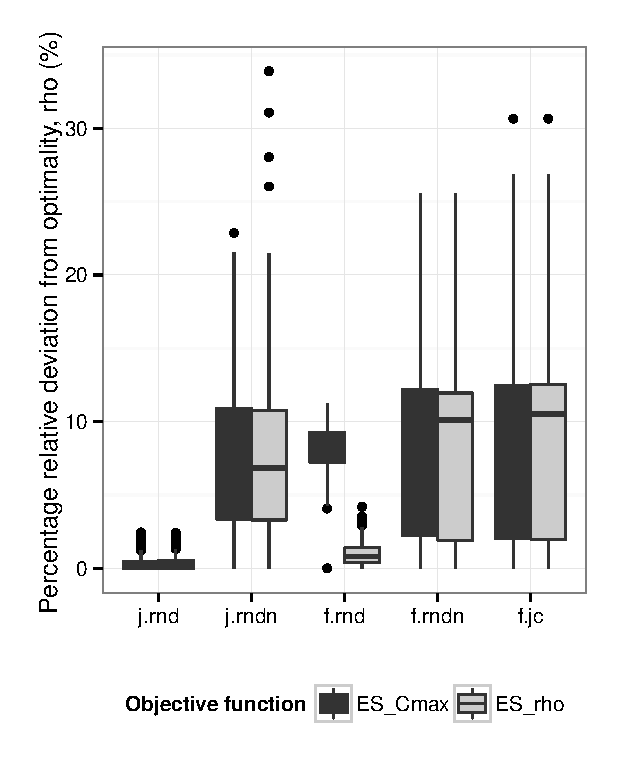
\epsfig{file=fig/CMAboxplotEvoTrain,width=\columnwidth}
\caption{Box-plot of training data for percentage relative deviation from optimality, defined by~\cref{eq:ratio}, when implementing the final weights obtained from CMA-ES optimisation, using both objective functions from~\cref{eq:cma:makespan,eq:cma:rho}, left and right, respectively.}\label{fig:cma:trainboxpl}
\end{figure}



\subsection{Problem difficulty}\label{sec:expr:data}
The evolution of fitness per generation from the CMA-ES optimisation of~\cref{eq:cma:rho} is depicted in~\cref{fig:cma:fit}. Note, all problem spaces reached their allotted computational time without converging. In fact $\mathcal{P}_{f.rnd}$ and $\mathcal{P}_{j.rndn}$ needed restarting during the optimisation process. 
Furthermore, the  evolution of the decision variables $\vec{w}$ are depicted in~\cref{fig:cma:wei}. As one can see, the relative contribution for each weight clearly differs between problem spaces. Note, that in the case of $\mathcal{P}_{j.rndn}$ (cf.~\cref{fig:cma:wei:rho}), CMA-ES restarts around generation 1,000 and quickly converges back to its previous fitness. However, lateral relation of weights has completely changed, implying that there are many optimal combinations of weights to be used. This can be expected due  to the fact some features in~\cref{tbl:jssp:feat} are a linear combination of others, e.g. $\phi_3=\phi_1+\phi_2$.

\begin{figure} % spans two columns
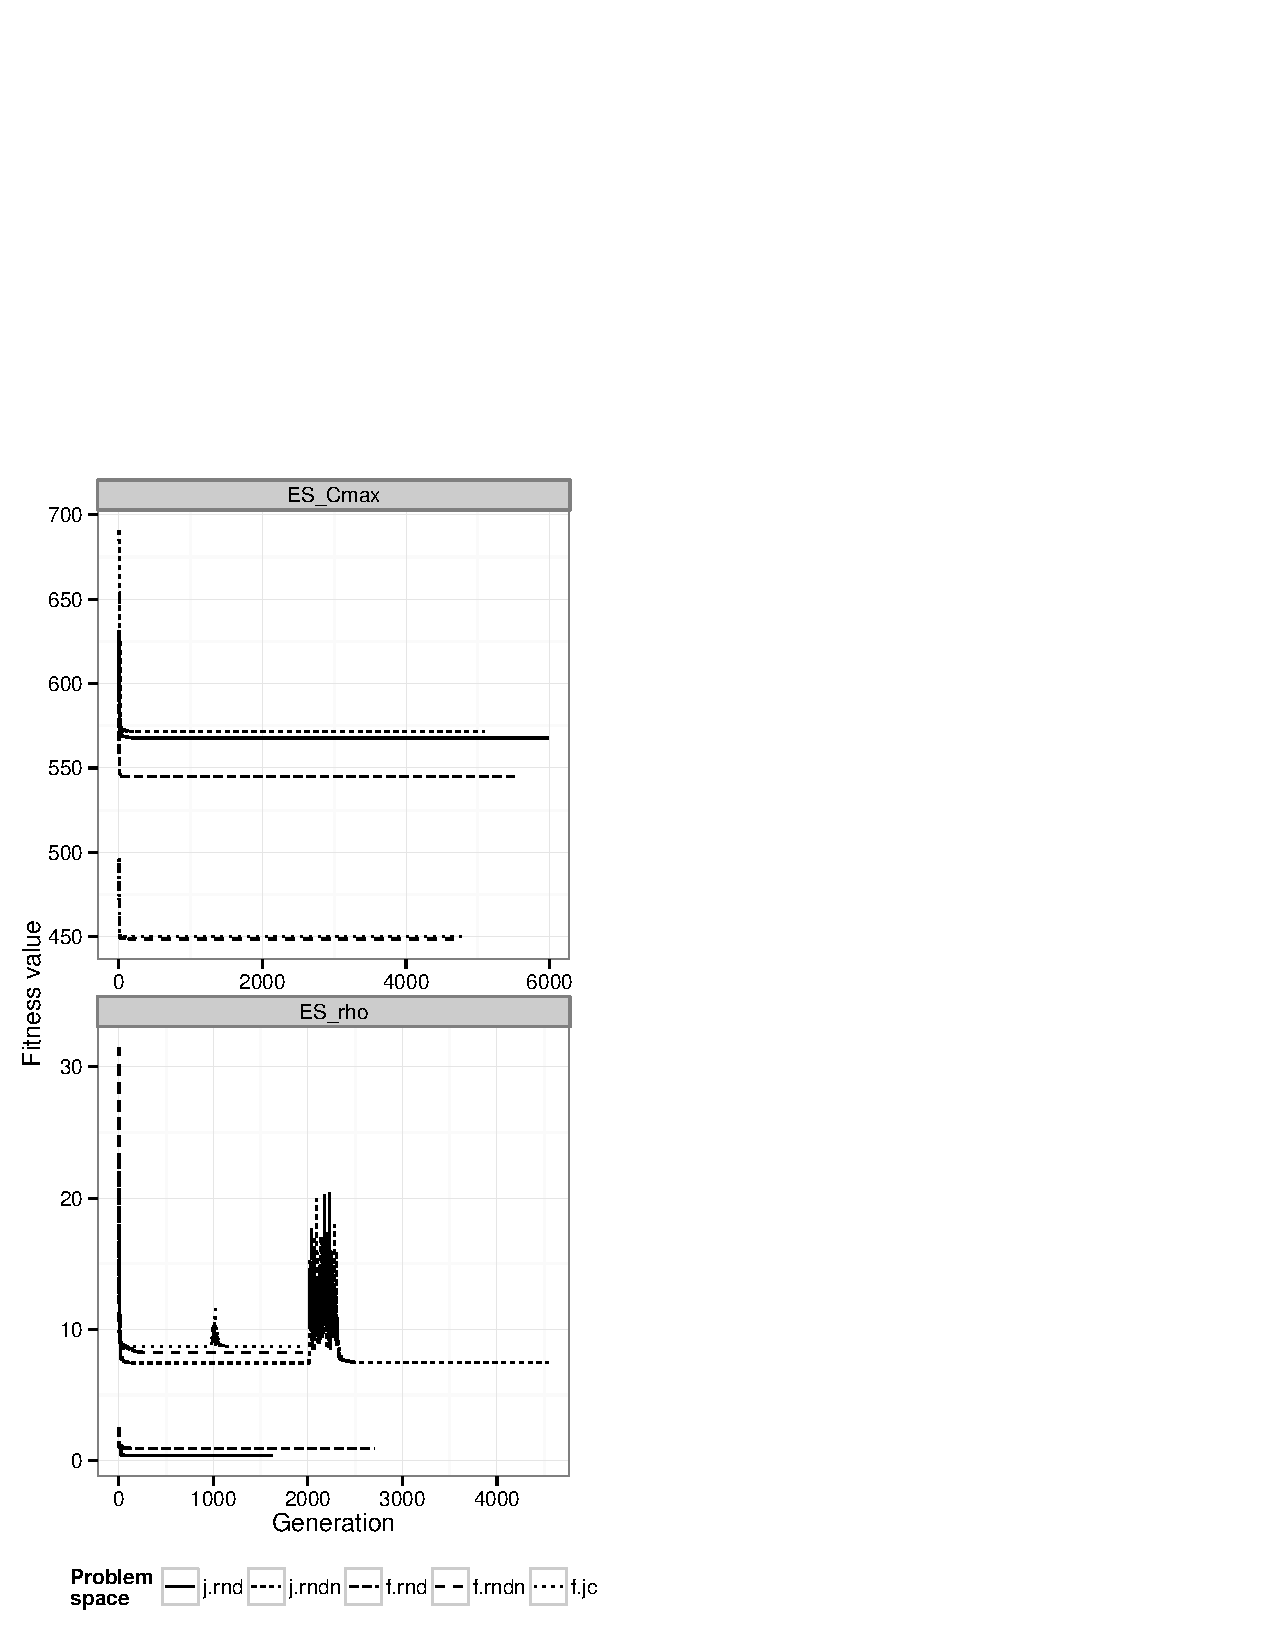
\epsfig{file=fig/CMAfitnessEvo, width=\columnwidth}
\caption{Fitness for optimising (w.r.t.~\cref{eq:cma:makespan,eq:cma:rho} above and below, receptively), per generation of the CMA-ES optimisation.}\label{fig:cma:fit}
\end{figure}


\begin{table*}\centering
\caption{Final results for CMA-ES optimisation; total number of generations and function evaluations and its resulting fitness value for both performance measures considered.}\label{cma:funeval}

\subtable[][w.r.t.~\cref{eq:cma:makespan}]{
\begin{tabular}{lrrr}\toprule
$\mathcal{P}$ & \#gen & \#eval & ES$_{C_{\max}}$ \\
\midrule
j.rnd & 4707 & 51788 & 448.612\\
j.rndn & 4802 & 52833 & 449.942 \\
f.rnd & 5088 & 55979 & 571.394 \\
f.rndn & 5557 & 61138 & 544.764 \\
f.jc & 5984 & 65835 & 567.688  \\
\bottomrule
\end{tabular}
}
\quad
\subtable[][w.r.t.~\cref{eq:cma:rho}]{
\begin{tabular}{lrrr}\toprule
$\mathcal{P}$ & \#gen & \#eval & ES$_\rho$ \\
\midrule
j.rnd & 1944 & 21395 & 8.258 \\
j.rndn & 1974 & 21725 & 8.691 \\
f.rnd & 4546 & 50006 & 7.479 \\
f.rndn & 2701 & 29722 & 0.938 \\
f.jc & 1625 & 17886 & 0.361 \\
\bottomrule
\end{tabular}
}

\end{table*}



\begin{figure*} \centering
\subfigure[][minimise w.r.t.~\cref{eq:cma:makespan}]{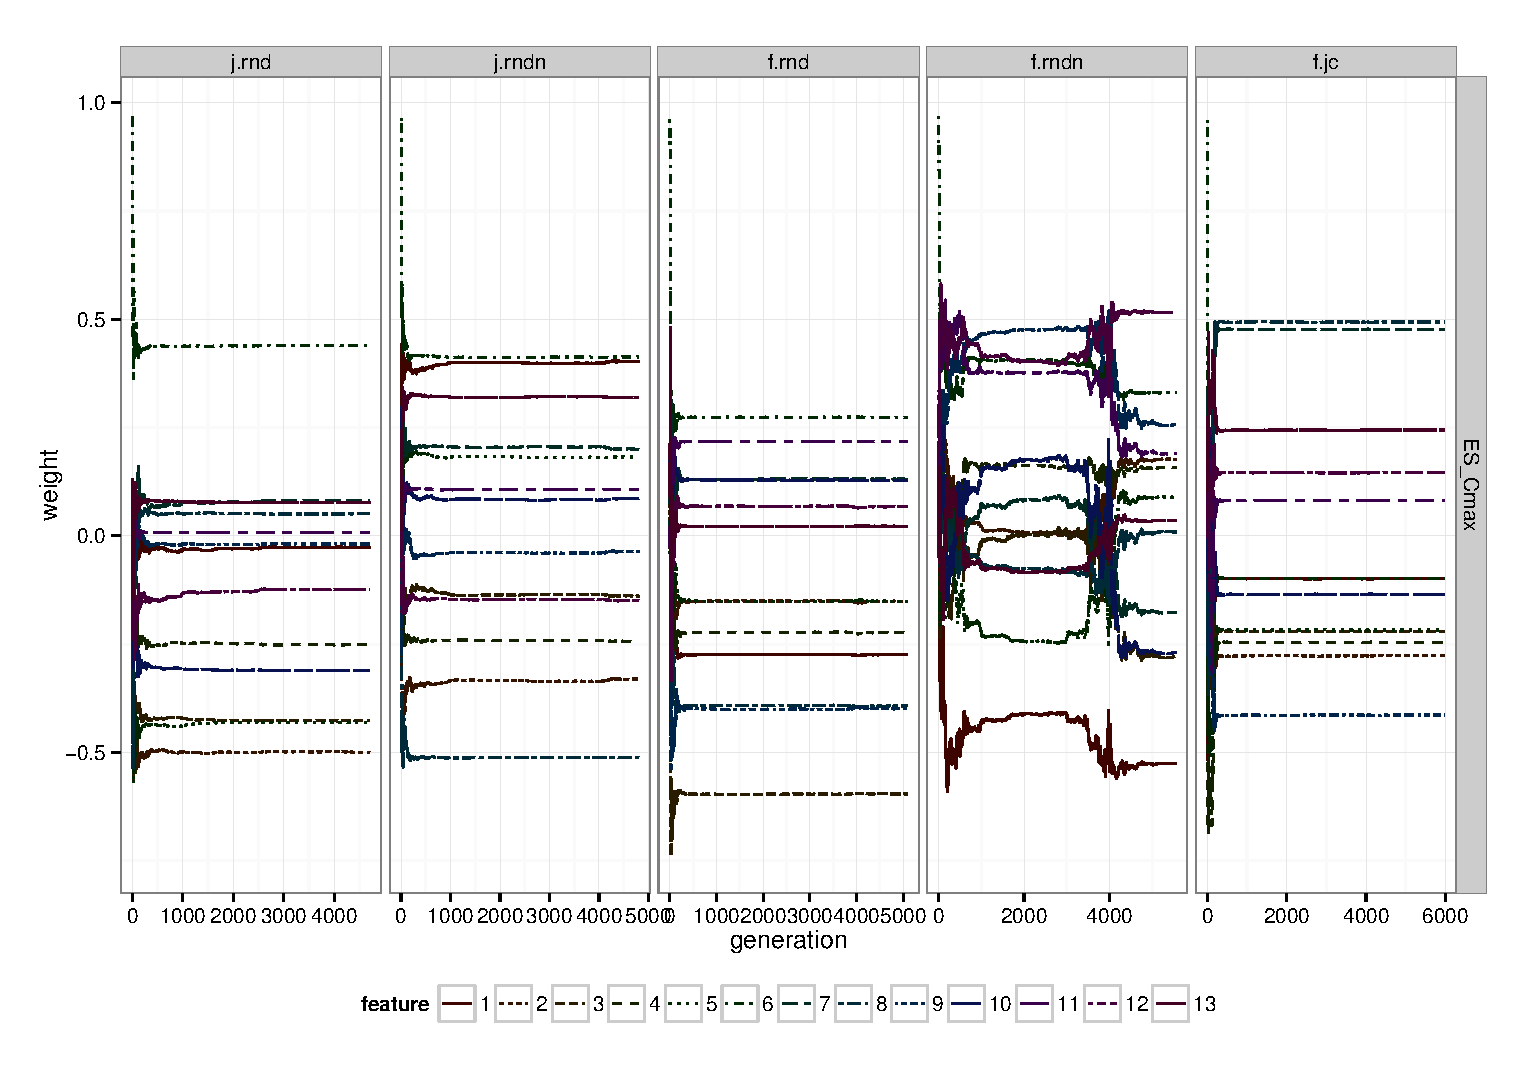
\epsfig{file={fig/CMAweightsEvo.ES_Cmax}.eps, width=\textwidth}\label{fig:cma:wei:cmax}}
\\
\subfigure[][minimise w.r.t.~\cref{eq:cma:rho}]{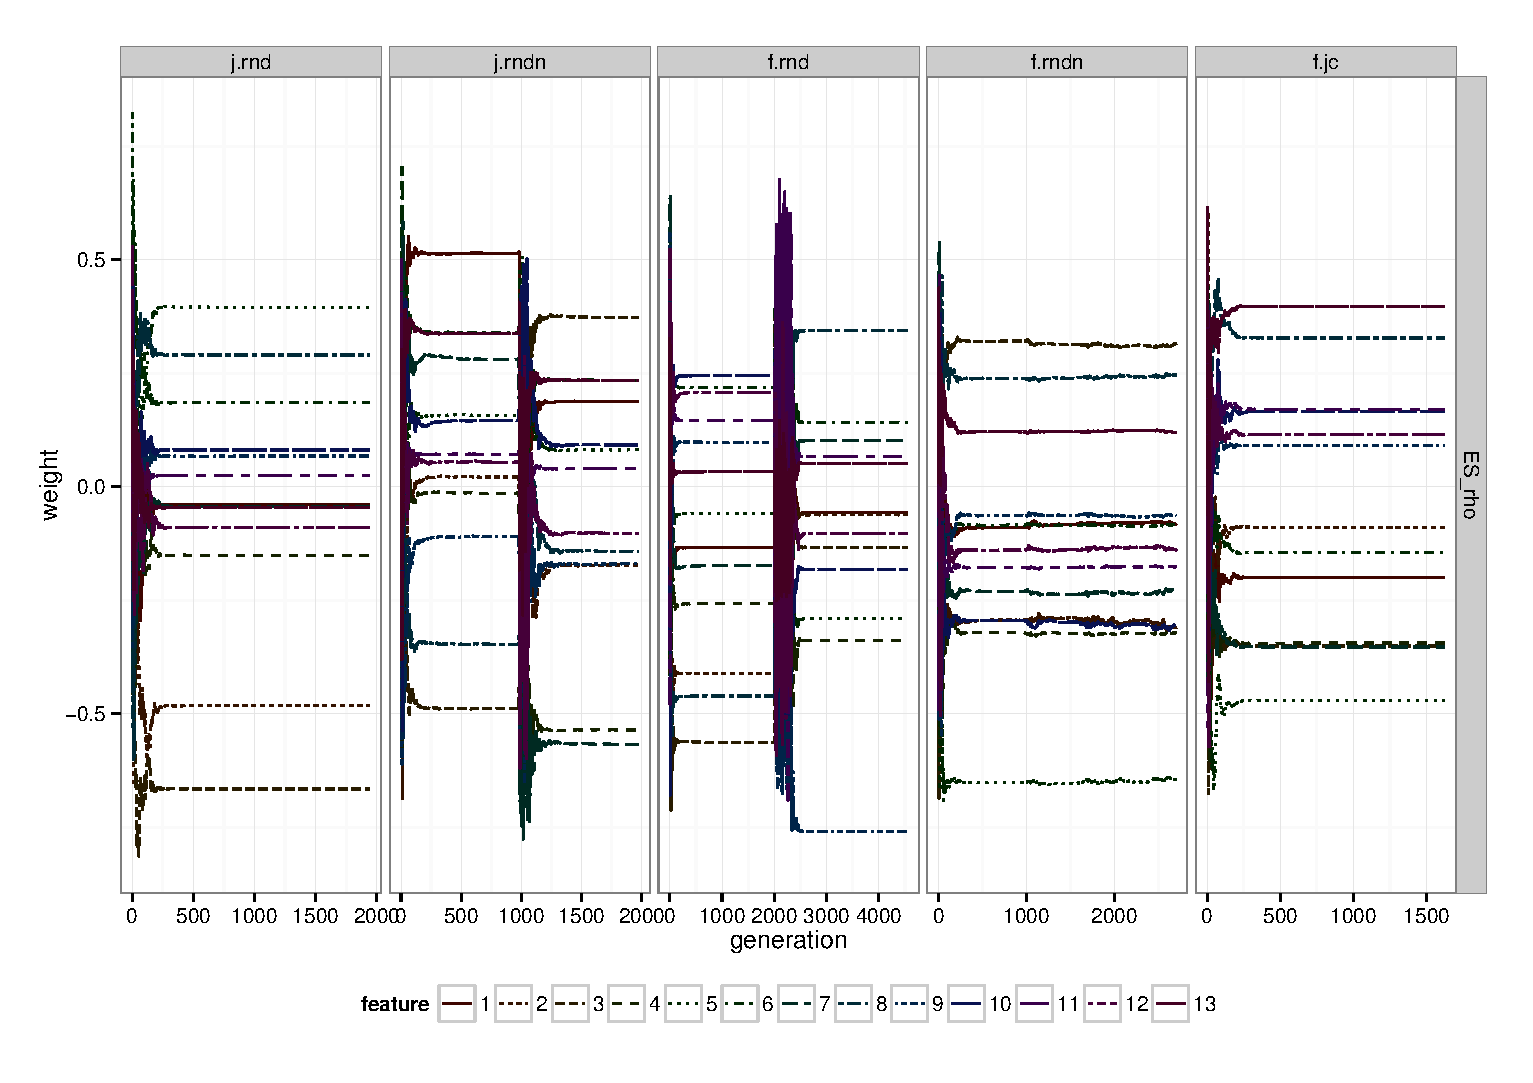
\epsfig{file={fig/CMAweightsEvo.ES_rho}.eps, width=\textwidth}\label{fig:cma:wei:rho}}
\caption{Evolution of weights of features (given in~\cref{tbl:jssp:feat}) at each generation of the CMA-ES optimisation. Note, weights are normalised such that $\norm{\vec{w}}=1$.}\label{fig:cma:wei}
\end{figure*}


\subsection{Scalability}\label{sec:expr:scalability} 
As a benchmark, the linear ordinal regression model (PREF) from~\cite{InRu11a} was created.
Using the weights obtained from optimising~\cref{eq:cma:rho} and applying them on their  $6\times5$ training data. Their main statistics of~\cref{eq:ratio} are reported in~\cref{tbl:results:train} for all training sets described in~\cref{tbl:data:sim}. Moreover, the best SDR from which the features in~\cref{tbl:jssp:feat} were inspired by, are also reported for comparison, i.e., most work remaining (MWR) for all JSP problem spaces, and least work remaining (LWR) for all PFSP problem spaces.

To explore the scalability of the learning models, a similar comparison to~\cref{sec:expr:data} is made for applying the learning models on their corresponding $10\times10$ testing data. Results are reported in~\cref{tbl:results:test}. Note, that only resulting $C_{\max}$ is reported as the optimum makespan is not known and~\cref{eq:ratio} is not applicable. 


\begin{table}[p]\centering
\caption{Main statistics of percentage relative deviation from optimality, $\rho$, defined by~\cref{eq:ratio} for various models, using corresponding $6\times5$ training data.}
\label{tbl:results:train}
%jsp
\subtable[][$\mathcal{P}_{ j.rnd }^{6\times5}$]{\label{tbl:train:j.rnd}
\begin{tabular}{lrrrrr} \toprule
model&mean & med & sd & min & max \\   \midrule
ES$_{C_{\max}}$& 8.54 & 10 &  6 &  0 & 26   \\ % CMA-ES min_Cmax j.rnd 6x5 train
ES$_\rho$& 8.26 & 10 &  6 &  0 & 26   \\ % CMA-ES min_rho j.rnd 6x5 train
PREF&   10.18 & 11 &  7 &  0 & 30  \\ %PREF j.rnd 6x5 train
MWR &  16.48 & 16 &  9 &  0 & 45   \\ %MWR j.rnd 6x5 train
\bottomrule \end{tabular}}
\\
\subtable[][$\mathcal{P}_{ j.rndn }^{6\times5}$]{\label{tbl:train:j.rndn}
\begin{tabular}{lrrrrr} \toprule
model&mean & med & sd & min & max \\   \midrule
ES$_{C_{\max}}$& 8.68 & 11 &  6 &  0 & 31   \\ % CMA-ES min_Cmax j.rndn 6x5 train
ES$_\rho$& 8.69 & 11 &  6 &  0 & 31   \\ % CMA-ES min_rho j.rndn 6x5 train
PREF&  10.00 & 11 &  6 &  0 & 31   \\ %PREF j.rndn 6x5 train
MWR &  14.02 & 13 &  8 &  0 & 37   \\ %MWR j.rndn 6x5 train
\bottomrule \end{tabular}}
%flow shop
\\
\subtable[][$\mathcal{P}_{ f.rnd }^{6\times5}$]{\label{tbl:train:f.rnd}
\begin{tabular}{lrrrrr} \toprule
model&mean & med & sd & min & max \\   \midrule
ES$_{C_{\max}}$& 7.44 &  7 &  5 &  0 & 23   \\ % CMA-ES min_Cmax f.rnd 6x5 train
ES$_\rho$& 7.48 &  7 &  5 &  0 & 34   \\ % CMA-ES min_rho f.rnd 6x5 train
PREF&   9.87 &  9 &  7 &  0 & 38  \\ %PREF f.rnd 6x5 train
LWR &  20.05 & 19 & 10 &  0 & 71   \\ %LWR f.rnd 6x5 train
\bottomrule \end{tabular}}
\\
\subtable[][$\mathcal{P}_{ f.rndn }^{6\times5}$]{\label{tbl:train:f.rndn}
\begin{tabular}{lrrrrr} \toprule
model&mean & med & sd & min & max \\   \midrule
ES$_{C_{\max}}$& 8.09 &  8 &  2 &  0 & 11   \\ % CMA-ES min_Cmax f.rndn 6x5 train
ES$_\rho$& 0.94 &  1 &  1 &  0 &  4   \\ % CMA-ES min_rho f.rndn 6x5 train
PREF&   2.38 &  2 &  1 &  0 &  7  \\ %PREF f.rndn 6x5 train
LWR &  2.25 &  2 &  1 &  0 &  7   \\ %LWR f.rndn 6x5 train
\bottomrule \end{tabular}}
\\
\subtable[][$\mathcal{P}_{ f.jc }^{6\times5}$]{\label{tbl:train:f.jc}
\begin{tabular}{lrrrrr} \toprule
model&mean & med & sd & min & max \\   \midrule
ES$_{C_{\max}}$& 0.33 &  0 &  0 &  0 &  2   \\ % CMA-ES min_Cmax f.jc 6x5 train
ES$_\rho$& 0.36 &  0 &  0 &  0 &  2   \\ % CMA-ES min_rho f.jc 6x5 train
PREF&   1.08 &  1 &  1 &  0 &  5  \\ %PREF f.jc 6x5 train
LWR &  1.13 &  1 &  1 &  0 &  6   \\ %LWR f.jc 6x5 train
\bottomrule \end{tabular}}
\end{table}

\begin{table}[p]\centering
\caption{Main statistics of $C_{\max}$ for various models, using corresponding $10\times 10$ test data. \newline}
\label{tbl:results:test}
%jsp
\subtable[][$\mathcal{P}_{ j.rnd }^{10\times10}$]{\label{tbl:test:j.rnd}
\begin{tabular}{lrrrrr}
  \toprule
model&mean & med & sd & min & max \\ 
  \midrule
ES$_{C_{\max}}$& 922.51 & 914 & 73 & 741 & 1173   \\ % CMA-ES min_Cmax j.rnd 10x10 test
ES$_\rho$& 931.37 & 931 & 71 & 735 & 1167   \\ % CMA-ES min_rho j.rnd 10x10 test
  PREF&   1011.38 & 1004 & 82 & 809 & 1281 \\   %PREF j.rnd 10x10 test
  MWR &  997.01 & 992 & 81 & 800 & 1273   \\ %MWR j.rnd 10x10 test
\bottomrule \end{tabular}}
\\
\subtable[][$\mathcal{P}_{ j.rndn }^{10\times10}$]{\label{tbl:test:j.rndn}
\begin{tabular}{lrrrrr}
  \toprule
model& mean & med & sd & min & max \\ 
  \midrule
ES$_{C_{\max}}$& 855.85 & 857 & 50 & 719 & 1010   \\ % CMA-ES min_Cmax j.rndn 10x10 test
ES$_\rho$& 855.91 & 856 & 51 & 719 & 1020   \\ % CMA-ES min_rho j.rndn 10x10 test
  PREF&   899.94 & 898 & 56 & 769 & 1130  \\ %PREF j.rndn 10x10 test
  MWR&  897.39 & 898 & 56 & 765 & 1088   \\ %MWR j.rndn 10x10 test
\bottomrule \end{tabular}}
%flow shop
\\
\subtable[][$\mathcal{P}_{ f.rnd }^{10\times10}$]{\label{tbl:test:f.rnd}
\begin{tabular}{lrrrrr} \toprule
model&mean & med & sd & min & max \\   \midrule
ES$_{C_{\max}}$& 1178.73 & 1176 & 80 & 976 & 1416   \\ % CMA-ES min_Cmax f.rnd 10x10 test
ES$_\rho$& 1181.91 & 1179 & 80 & 984 & 1404   \\ % CMA-ES min_rho f.rnd 10x10 test
PREF&  1215.20 & 1212 & 80 & 1006 & 1450  \\ %PREF f.rnd 10x10 test
LWR &  1284.41 & 1286 & 85 & 1042 & 1495   \\ %LWR f.rnd 10x10 test
\bottomrule \end{tabular}}
\\
\subtable[][$\mathcal{P}_{ f.rndn }^{10\times10}$]{\label{tbl:test:f.rndn}
\begin{tabular}{lrrrrr} \toprule
model&mean & med & sd & min & max \\   \midrule
ES$_{C_{\max}}$& 1065.48 & 1059 & 32 & 992 & 1222   \\ % CMA-ES min_Cmax f.rndn 10x10 test
ES$_\rho$& 980.11 & 980 &  8 & 957 & 1006   \\ % CMA-ES min_rho f.rndn 10x10 test
PREF&  987.49 & 988 &  9 & 958 & 1011  \\ %PREF f.rndn 10x10 test
LWR &  986.94 & 987 &  9 & 959 & 1010   \\ %LWR f.rndn 10x10 test
\bottomrule \end{tabular}}
\\
\subtable[][$\mathcal{P}_{ f.jc }^{10\times10}$]{\label{tbl:test:f.jc}
\begin{tabular}{lrrrrr} \toprule
model&mean & med & sd & min & max \\   \midrule
ES$_{C_{\max}}$& 1135.44 & 1134 & 286 & 582 & 1681   \\ % CMA-ES min_Cmax f.jc 10x10 test
ES$_\rho$& 1135.47 & 1134 & 286 & 582 & 1681   \\ % CMA-ES min_rho f.jc 10x10 test
PREF&   1136.02 & 1135 & 286 & 582 & 1685 \\  %PREF f.jc 10x10 test
LWR &  1136.49 & 1141 & 287 & 581 & 1690   \\ %LWR f.jc 10x10 test
\bottomrule \end{tabular}}

\end{table}

\section{\uppercase{Discussion and conclusions}}\label{sec:disc}
Data distributions considered in this study either varied 
w.r.t. the processing time distributions, continuing the preliminary experiments in ~\cite{InRu11a} , or 
w.r.t. the job ordering permutations -- i.e., homogeneous machine order for PFSP versus heterogeneous machine order for JSP. 
From the results based on $6\times5$ training data given  in~\cref{tbl:results:train}, it's obvious that CMA-ES optimisation substantially outperforms the previous PREF methods from~\cite{InRu11a} for all problem spaces considered. Furthermore, the results hold when testing on $10\times10$ (cf.~\cref{tbl:results:test}), suggesting the method is indeed  scalable for higher dimensions. 

Moreover, the study showed that the choice of objective function  for evolutionary search is worth investigating. There was no statistical difference from minimising the fitness function directly and its normalisation w.r.t. true optimum (cf.~\cref{eq:cma:makespan,eq:cma:rho}), save for $\mathcal{P}_{f.rndn}$. Implying, even though ES doesn't rely on optimal solutions, there are some problem spaces where it can be of great benefit. This is due to the fact that the problem instances can vary greatly within the same problem space \cite{InRu12}. Thus normalising the objective function would help the evolutionary search to deviate the from giving too much weight for problematic problem instances for the greater good.

%The weights for~\cref{eq:jssp:linweights} in~\cite{InRu11a} were found using supervised learning, where the training data was created from optimal solutions of randomly generated problem instances. As an alternative, this study showed  that minimising the mean makespan directly using a brute force search via CMA-ES actually results in a better CDRs. The nature of CMA-ES is to explore suboptimal routes until it converges to an optimal one. Implying that the previous approach of only looking into one optimal route may not produce a sufficiently rich training set. That is, the training set should incorporate a more complete knowledge on \emph{all} possible preferences, i.e., make also the distinction between suboptimal and sub-suboptimal features, etc.  This would require a Pareto ranking of preferences which can be used to make the distinction to which feature sets are equivalent, better or worse -- and to what degree, i.e., by giving a weight to the preference. This would result in a very large training set, which of course could be re-sampled in order to make it computationally feasible to learn.

The main drawback of using evolutionary search for learning optimal weights for~\cref{eq:jssp:linweights} is how computationally expensive it is to evaluate the mean expected fitness. Even for a low problem dimension 6-job 5-machine JSP, each optimisation run reached their walltime of 288 hours without converging. Now, $6\times5$ JSP requires 30 sequential operations where at each time step there are up to $6$ jobs to choose from -- i.e., its complexity is $\mathcal{O}(n^{n\cdot m})$ making it computationally infeasible to apply this framework for higher dimensions as is. 
However, evolutionary search only requires the rank of the candidates and therefore it is appropriate to retain a sufficiently accurate surrogate for the value function during evolution in order to reduce the number of costly true value function evaluations, such as the approach in~\cite{InRu11b}. This could reduce the computational cost of the evolutionary search considerably, making it feasible to conduct the experiments from~\cref{sec:expr} for problems of higher dimensions, e.g. with these adjustments it is possible to train on $10\times10$ and test on for example $14\times14$ to verify whether scalability holds for even higher dimensions.  


\clearpage
\bibliographystyle{apalike}
{\small

%\bibliography{../references}
\begin{thebibliography}{}

\bibitem[Ak and Koc, 2012]{Ak12}
Ak, B. and Koc, E. (2012).
\newblock {A Guide for Genetic Algorithm Based on Parallel Machine Scheduling
  and Flexible Job-Shop Scheduling}.
\newblock {\em Procedia - Social and Behavioral Sciences}, 62:817--823.

\bibitem[Burke et~al., 2013]{Burke10}
Burke, E.~K., Gendreau, M., Hyde, M., Kendall, G., Ochoa, G., Ozcan, E., and
  Qu, R. (2013).
\newblock Hyper-heuristics: a survey of the state of the art.
\newblock {\em Journal of the Operational Research Society}, 64(12):1695--1724.

\bibitem[Cheng et~al., 1996]{Cheng96}
Cheng, R., Gen, M., and Tsujimura, Y. (1996).
\newblock {A tutorial survey of job-shop scheduling problems using genetic
  algorithms—I. Representation}.
\newblock {\em Computers \& Industrial Engineering}, 30(4):983--997.

\bibitem[Cheng et~al., 1999]{Cheng99}
Cheng, R., Gen, M., and Tsujimura, Y. (1999).
\newblock {A tutorial survey of job-shop scheduling problems using genetic
  algorithms, part II: hybrid genetic search strategies}.
\newblock {\em Computers \& Industrial Engineering}, 36(2):343--364.

\bibitem[Dhingra and Chandna, 2010]{Dhingra10}
Dhingra, A. and Chandna, P. (2010).
\newblock {A bi-criteria M-machine SDST flow shop scheduling using modified
  heuristic genetic algorithm}.
\newblock {\em International Journal of Engineering, Science and Technology},
  2(5):216--225.

\bibitem[{Gurobi Optimization, Inc.}, 2013]{gurobi}
{Gurobi Optimization, Inc.} (2013).
\newblock Gurobi optimization (version 5.6.2) [software].

\bibitem[Hansen and Ostermeier, 2001]{Hansen01}
Hansen, N. and Ostermeier, A. (2001).
\newblock Completely derandomized self-adaptation in evolution strategies.
\newblock {\em Evol. Comput.}, 9(2):159--195.

\bibitem[Haupt, 1989]{Haupt89}
Haupt, R. (1989).
\newblock A survey of priority rule-based scheduling.
\newblock {\em OR Spectrum}, 11:3--16.

\bibitem[Ingimundardottir and Runarsson, 2011a]{InRu11b}
Ingimundardottir, H. and Runarsson, T.~P. (2011a).
\newblock Sampling strategies in ordinal regression for surrogate assisted
  evolutionary optimization.
\newblock In {\em Intelligent Systems Design and Applications (ISDA), 2011 11th
  International Conference on}, pages 1158--1163.

\bibitem[Ingimundardottir and Runarsson, 2011b]{InRu11a}
Ingimundardottir, H. and Runarsson, T.~P. (2011b).
\newblock Supervised learning linear priority dispatch rules for job-shop
  scheduling.
\newblock In Coello, C., editor, {\em Learning and Intelligent Optimization},
  volume 6683 of {\em Lecture Notes in Computer Science}, pages 263--277.
  Springer, Berlin, Heidelberg.

\bibitem[Ingimundardottir and Runarsson, 2012]{InRu12}
Ingimundardottir, H. and Runarsson, T.~P. (2012).
\newblock Determining the characteristic of difficult job shop scheduling
  instances for a heuristic solution method.
\newblock In Hamadi, Y. and Schoenauer, M., editors, {\em Learning and
  Intelligent Optimization}, Lecture Notes in Computer Science, pages 408--412.
  Springer, Berlin, Heidelberg.

\bibitem[Jayamohan and Rajendran, 2004]{Jayamohan04}
Jayamohan, M. and Rajendran, C. (2004).
\newblock Development and analysis of cost-based dispatching rules for job shop
  scheduling.
\newblock {\em European Journal of Operational Research}, 157(2):307--321.

\bibitem[Koza and Poli, 2005]{Koza05}
Koza, J.~R. and Poli, R. (2005).
\newblock {Genetic programming}.
\newblock In Burke, E. and Kendal, G., editors, {\em Introductory Tutorials in
  Optimization and Decision Support Techniques}, chapter~5. Springer.

\bibitem[Nguyen et~al., 2013]{Nguyen13}
Nguyen, S., Zhang, M., Johnston, M., and Tan, K.~C. (2013).
\newblock {Learning iterative dispatching rules for job shop scheduling with
  genetic programming}.
\newblock {\em The International Journal of Advanced Manufacturing Technology}.

\bibitem[Panwalkar and Iskander, 1977]{Panwalkar77}
Panwalkar, S.~S. and Iskander, W. (1977).
\newblock A survey of scheduling rules.
\newblock {\em Operations Research}, 25(1):45--61.

\bibitem[Pinedo, 2008]{Pinedo08}
Pinedo, M.~L. (2008).
\newblock {\em Scheduling: Theory, Algorithms, and Systems}.
\newblock Springer Publishing Company, Incorporated, 3 edition.

\bibitem[Qing-dao-er ji and Wang, 2012]{Qing-dao-er-ji12}
Qing-dao-er ji, R. and Wang, Y. (2012).
\newblock {A new hybrid genetic algorithm for job shop scheduling problem}.
\newblock {\em Computers \& Operations Research}, 39(10):2291--2299.

\bibitem[Rice, 1976]{Rice76}
Rice, J.~R. (1976).
\newblock The algorithm selection problem.
\newblock {\em Advances in Computers}, 15:65--118.

\bibitem[Smith-Miles et~al., 2009]{SmithMilesLion3}
Smith-Miles, K., James, R., Giffin, J., and Tu, Y. (2009).
\newblock A knowledge discovery approach to understanding relationships between
  scheduling problem structure and heuristic performance.
\newblock In Stützle, T., editor, {\em Learning and Intelligent Optimization},
  volume 5851 of {\em Lecture Notes in Computer Science}, pages 89--103.
  Springer, Berlin, Heidelberg.

\bibitem[Smith-Miles and Lopes, 2011]{SmithMilesLion5}
Smith-Miles, K. and Lopes, L. (2011).
\newblock Generalising algorithm performance in instance space: A timetabling
  case study.
\newblock In Coello, C., editor, {\em Learning and Intelligent Optimization},
  volume 6683 of {\em Lecture Notes in Computer Science}, pages 524--538.
  Springer, Berlin, Heidelberg.

\bibitem[Tay and Ho, 2008]{Tay08}
Tay, J.~C. and Ho, N.~B. (2008).
\newblock Evolving dispatching rules using genetic programming for solving
  multi-objective flexible job-shop problems.
\newblock {\em Computers and Industrial Engineering}, 54(3):453--473.

\bibitem[Tsai et~al., 2007]{Tsai07}
Tsai, J.-T., Liu, T.-K., Ho, W.-H., and Chou, J.-H. (2007).
\newblock {An improved genetic algorithm for job-shop scheduling problems using
  Taguchi-based crossover}.
\newblock {\em The International Journal of Advanced Manufacturing Technology},
  38(9-10):987--994.

\bibitem[V\'{a}zquez-Rodr\'{\i}guez and Petrovic, 2009]{Vazquez-Rodriguez09}
V\'{a}zquez-Rodr\'{\i}guez, J.~A. and Petrovic, S. (2009).
\newblock {A new dispatching rule based genetic algorithm for the
  multi-objective job shop problem}.
\newblock {\em Journal of Heuristics}, 16(6):771--793.

\bibitem[Watson et~al., 2002]{Whitley}
Watson, J.-P., Barbulescu, L., Whitley, L.~D., and Howe, A.~E. (2002).
\newblock Contrasting structured and random permutation flow-shop scheduling
  problems: Search-space topology and algorithm performance.
\newblock {\em INFORMS Journal on Computing}, 14:98--123.

\end{thebibliography}

}


\end{document}

